\documentclass[twoside,a4paper]{article}
\usepackage{geometry}
\geometry{margin=1.5cm, vmargin={0pt,1cm}}
\setlength{\topmargin}{-1cm}
\setlength{\paperheight}{29.7cm}
\setlength{\textheight}{25.3cm}

% useful packages.
\usepackage{amsfonts}
\usepackage{amsmath}
\usepackage{amssymb}
\usepackage{amsthm}
\usepackage{enumerate}
\usepackage{graphicx}
\usepackage{multicol}
\usepackage{fancyhdr}
\usepackage{layout}
\usepackage{listings}
\usepackage{float, caption}
\usepackage{xeCJK}

\lstset{
    basicstyle=\ttfamily, basewidth=0.5em
}

% some common command
\newcommand{\dif}{\mathrm{d}}
\newcommand{\avg}[1]{\left\langle #1 \right\rangle}
\newcommand{\difFrac}[2]{\frac{\dif #1}{\dif #2}}
\newcommand{\pdfFrac}[2]{\frac{\partial #1}{\partial #2}}
\newcommand{\OFL}{\mathrm{OFL}}
\newcommand{\UFL}{\mathrm{UFL}}
\newcommand{\fl}{\mathrm{fl}}
\newcommand{\op}{\odot}
\newcommand{\Eabs}{E_{\mathrm{abs}}}
\newcommand{\Erel}{E_{\mathrm{rel}}}

\begin{document}

\pagestyle{fancy}
\fancyhead{}
\lhead{Wenchong Huang (3200100006)}
\chead{Numerical PDE homework \#4}
\rhead{May.7th, 2023}

\section*{I. Exercise 11.159 (显式中点法的一步误差表示)}

\;\;\;\;\;\;图中红色加粗线段确实是显式中点法的一步误差。注意到$l_1$的斜率为$f(U^n,t_n)=y_1$, $l_2$与$l_3$的斜率为$f(U^n+\frac{k}{2}y_1,t_n+\frac{k}{2})=y_2$,从而$l_3$在$t_{n+1}$处的取值为:
\begin{equation*}
    U^n+ky_2=U^{n+1}.
\end{equation*}

从而红色加粗线段表示:
\begin{equation*}
    U^{n+1}-U^n-(u(t_{n+1})-u(t_n))=-\mathcal{L}u(t_n).
\end{equation*}

其长度恰好为一步误差的绝对值。

\section*{II. Exercise 11.161 (TR-BDF2法的一步误差表示)}

\;\;\;\;\;\;第一步的示意图如下:

如图,$l_1$的斜率为$f(U^n,t_n)$,$l_3$的斜率为$f(U^*,t_n+\frac{k}{2})$,$l_2$的斜率为$l_1$与$l_3$斜率的平均值,为确定$U^*$的位置,需要保证$l_2$过$U^n$.

\begin{figure}[H]
    \centering
    \includegraphics[width=0.3\textwidth]{figures/161-1.png}
\end{figure}

第二步的计算可以表示为:
\begin{equation*}
    U^{n+1}=U^n+\frac{k}{3}\left(f(U^n,t_n)+f(U^*,t_k+\frac{k}{2})+f(U^{n+1},t_{n+1})\right).
\end{equation*}

\section*{III. Exercise 11.165 (显式中点法的阶数)}

\;\;\;\;\;\;注意到$y_1=f$,对于$y_2$,由泰勒展开:
\begin{align*}
    y_2 &= f+\frac{k}{2}y_1f_u+\frac{k}{2}f_t+\frac{k^2}{8}y_1^2f_{uu}+\frac{k^2}{4}y_1f_{ut}+\frac{k^2}{8}f_{tt}\\
    &= u' + \frac{k}{2}u'' + \frac{k^2}{8}(u'''-f_uu'') + O(k^3).
\end{align*}

从而得到一步误差:
\begin{align*}
    \mathcal{L}u(t(n))&=(u + ku'+\frac{k^2}{2}u''+\frac{k^3}{6}u''')-u - ku' - k(u' + \frac{k}{2}u'' + \frac{k^2}{8}(u'''-f_uu'')) + O(k^4)\\
    &= \frac{k^3}{24}(u'''+3f_uu'') + O(k^4).
\end{align*}

所以$\mathcal{L}u(t_n)=\Theta(k^3)$,因此具有二阶精度。

\section*{IV. Exercise 11.174 (TR-BDF2法的稳定函数)}

\;\;\;\;\;\;根据TR-BDF2法的计算公式:
\begin{equation*}
    U^*=U^n+\frac{k}{4}(\lambda U^n + \lambda U^*) \implies U^*=\frac{1+z/4}{1-z/4}U^n.
\end{equation*}

\begin{align*}
    &U^{n+1}=\frac{1}{3}\left(4\frac{1+z/4}{1-z/4}U^n - U^n + zU^{n+1}\right)\\
    \implies & U^{n+1}=\frac{1+\frac{5}{12}z}{(1-z/3)(1-z/4)}U^n=\frac{1+\frac{5}{12}z}{1-\frac{7}{12}z+\frac{1}{12}z^2}U^n.
\end{align*}

由定义即
\begin{equation*}
    R(z)=\frac{1+\frac{5}{12}z}{1-\frac{7}{12}z+\frac{1}{12}z^2}.
\end{equation*}

且有
\begin{align*}
    R(z)-e^z &= R(z) - (1+z+\frac{z^2}{2}) + O(z^3)\\
    &= \frac{1+\frac{5}{12}z - \left(1+z+\frac{1}{2}z^2\right)\left(1-\frac{7}{12}z+\frac{1}{12}z^2\right)}{1-\frac{7}{12}z+\frac{1}{12}z^2} + O(z^3)\\
    &= \frac{-\frac{5}{24}z^3+\frac{1}{24}z^4}{1-\frac{7}{12}z+\frac{1}{12}z^2}+O(z^3)\\
    &= O(z^3) \quad (z\to 0).
\end{align*}

\section*{V. Exercise 11.179 (向后欧拉方法和梯形方法求解刚性方程的稳定性)}

\;\;\;\;\;\;生成的表格如下:

\begin{lstlisting}
                    Backward Euler  Trapezoidal
    eta=1   k=0.2   9.77307e-08     4.72289e-10
            k=0.1   4.92233e-08     1.17719e-10
            k=0.05  2.46859e-08     2.94077e-11
    eta=1.5 k=0.2   9.77307e-08     0.49985
            k=0.1   4.92233e-08     0.4994
            k=0.05  2.46859e-08     0.497606
\end{lstlisting}

生成的图像如下:
\begin{figure}[H]
    \centering
    \begin{minipage}[t]{0.3\linewidth}
        \centering
        \includegraphics[width=0.95\linewidth]{figures/11-179-1.eps}
        \caption*{Backward Eular}
    \end{minipage}
    \hspace{2em}
    \begin{minipage}[t]{0.3\linewidth}
        \centering
        \includegraphics[width=0.95\linewidth]{figures/11-179-2.eps}
        \caption*{Trapezoidal}
    \end{minipage}
\end{figure}

我们直接采用了第11章编程题的程序,向后欧拉方法就是1阶BDF法,梯形方法就是2阶Adams-Moulton法。由于代码过长,这里不予展示。完整的代码文件已经放在\verb|programs/11-179|中,在目录中执行
\begin{lstlisting}
    make run
\end{lstlisting}

即可自动编译、自动运行,最终会生成表格的结果和两个图像。\textbf{注意:您需要安装gnuplot才能进行测试}。

为了解释上述原因,我们需要指出:在第一步求解中,向后欧拉方法求得了近乎精确的解,而梯形方法求得的解误差很大。将向后欧拉方法的表达式代入本题所求方程,得到:
\begin{equation*}
    U^1=\eta+k(\lambda(y-\cos k)-\sin k),
\end{equation*}

从而对于$\lambda=-10^6,\eta=1.5$,有:
\begin{equation*}
    U^1= \frac{\eta-k\lambda\cos k - k\sin k}{1-k\lambda}\approx \frac{-k\lambda\cos k}{1-k\lambda} \approx 1.
\end{equation*}

将梯形方法的表达式代入本题所求方程,得到:
\begin{equation*}
    U^1=\eta+\frac{k}{2}(\lambda(\eta-1)+\lambda(y-\cos k)-\sin k),
\end{equation*}

从而对于$\lambda=-10^6,\eta=1.5$,有:
\begin{equation*}
    U^1= \frac{\eta+\frac{k}{4}\lambda-\frac{k\lambda}{2}\cos k-\frac{k}{2}\sin k}{1-\frac{k\lambda}{2}}\approx \frac{\frac{k}{4}\lambda-\frac{k\lambda}{2}\cos k}{1-\frac{k\lambda}{2}}\approx 0.5
\end{equation*}

在此后的求解中,同理可以证明,当$U^n\approx u(t_n)\pm0.5$时,$U^{n+1}\approx u(t_{n+1})\mp0.5$,从而梯形方法的求解结果与真解一直保持大约$0.5$的误差。

\section*{VI. Exercise 11.182 (一些数值方法的Butcher表)}

\begin{table}[H]
    \renewcommand\arraystretch{1.2}
    \centering
    \begin{minipage}[t]{0.3\linewidth}
        \centering
        \begin{tabular}{l|ll}
            $0$           & $0$           &     \\
            $\frac{1}{2}$ & $\frac{1}{2}$ & $0$ \\ \hline
                        & $0$           & $1$
        \end{tabular}
        \caption*{修正欧拉方法(Modified Eular)}
    \end{minipage}
    \begin{minipage}[t]{0.3\linewidth}
        \centering
        \begin{tabular}{l|ll}
            $0$           & $0$           &     \\
            $1$ & $1$ & $0$ \\ \hline
                        & $\frac{1}{2}$           & $\frac{1}{2}$
        \end{tabular}
        \caption*{改良欧拉方法(Improved Eular)}
    \end{minipage}
    \begin{minipage}[t]{0.3\linewidth}
        \centering
        \begin{tabular}{l|lll}
            $0$           & $0$           &    &  \\
            $\frac{1}{3}$ & $\frac{1}{3}$ & $0$ & \\
            $\frac{2}{3}$ & $0$ & $\frac{2}{3}$ & $0$ \\ \hline
                        & $\frac{1}{4}$     & $0$      & $\frac{3}{4}$
        \end{tabular}
        \caption*{休恩方法(Heun)}
    \end{minipage}
\end{table}

\section*{VII. Exercise 11.183 (RK方法的另一种形式)}

\;\;\;\;\;\;令
\begin{equation*}
    \mathbf{\xi}_i=\mathbf{U}^n+k\sum_{j=1}^s a_{ij}\mathbf{y}_j,
\end{equation*}

则
\begin{equation*}
    \mathbf{\xi}_i=\mathbf{U}^n+k\sum_{j=1}^s a_{ij}\mathbf{f}(\mathbf{\xi}_j,t_n+c_jk),
\end{equation*}
\begin{equation*}
    \mathbf{U}^{n+1}=\mathbf{U}^n+k\sum_{j=1}^s b_j\mathbf{f}(\mathbf{\xi}_j,t_n+c_jk).
\end{equation*}

\section*{VIII. Exercise 11.190 (一族单参数三阶显式RK方法)}

设三阶显式RK方法的Butcher表为:

\begin{table}[H]
    \centering
    \begin{tabular}{l|lll}
        $0$           & $0$           &    &  \\
        $c_2$ & $a_{21}$ & $0$ & \\
        $c_3$ & $a_{31}$ & $a_{32}$ & $0$ \\ \hline
                    & $b_1$     & $b_2$      & $b_3$
    \end{tabular}
\end{table}

需要满足定理11.184中的条件:$a_{21}=c_2$,$a_{31}+a_{32}=c_3$,$b_1+b_2+b_3=1$. 我们设$b_3=\alpha$. 做泰勒展开,得到:
\begin{align*}
    y_2&=f+c_2kf_uf+c_2kf_t+\frac{k^2c_2^2}{2}(f_{uu}f^2+2ff_{ut}+f_{tt})+O(k^3)\\
    &=u'+c_2ku''+\frac{k^2c_2^2}{2}(u'''-f_uu'')+O(k^3)
\end{align*}
\begin{equation*}
    y_3=f+k(a_{31}f+a_{32}y_2)f_u+c_3kf_t+\frac{k^2}{2}(a_{31}f+a_{32}y_2)^2f_{uu}+\frac{1}{2}c_3^2k^2f_{tt}+c_3k^2(a_{31}f+a_{32}y_2)f_{ut}+O(k^3).
\end{equation*}

代入一步误差表达式,得到:
\begin{align*}
    \mathcal{L}u(t_n)&= ku'+\frac{k^2}{2}u''+\frac{k^3}{6}u'''-k(b_1f+b_2y_2+\alpha y_3) + O(k^4)\\
    &= \left(\frac{1}{2}-b_2c_2-\alpha c_3\right)k^2u''+\left(\frac{1}{6}-\frac{1}{2}c_2^2b_2-\frac{1}{2}\alpha c_3^2\right)k^3u''' + 
    \left(\frac{1}{2}b_2c_2^2 - \alpha a_{32}c_2 + \frac{1}{2}\alpha c_3^2\right)k^3 u''f_u + O(k^4).
\end{align*}

为保证三阶精度,我们需要下面的代数方程组得到满足:
\begin{equation*}
    \left\{\begin{array}{l}
        2b_2c_2+2\alpha c_3=1\\
        b_2c_2^2+\alpha c_3^2 = \frac{1}{3}\\
        b_2c_2^2-2\alpha a_{32}c_2 + \alpha c_3^2 = 0
    \end{array}\right.
\end{equation*}

令$c_2=c_3$,我们可以得到一组典型解:
\begin{equation*}
    c_2=c_3=\frac{2}{3},\quad b_2=\frac{3}{4}-\alpha,\quad a_{32}=\frac{1}{4\alpha}
\end{equation*}

再由定理11.184中的条件可以求得:
\begin{equation*}
    a_{31}=c_3-a_{32}=\frac{2}{3}-\frac{1}{4\alpha},\quad b_1=1-b_2-b_3=\frac{1}{4}.
\end{equation*}

这样我们就得到了一族单参数三阶精度的显式RK方法,其Butcher表为:

\begin{table}[H]
    \renewcommand\arraystretch{1.5}
    \centering
    \begin{tabular}{c|ccc}
        $0$           & $0$           &    &  \\
        $\frac{2}{3}$ & $\frac{2}{3}$ & $0$ & \\
        $\frac{2}{3}$ & $\frac{2}{3}-\frac{1}{4\alpha}$ & $\frac{1}{4\alpha}$ & $0$ \\ \hline
                    & $\frac{1}{4}$     & $\frac{3}{4}-\alpha$      & $\alpha$
    \end{tabular}
\end{table}

显然Heun方法不属于该族,因为它不满足$c_2=c_3$.

\section*{IX. Exercise 11.196 (证明积分公式对$r-1$阶多项式成立当且仅当RK方法满足$B(r)$性质)}

\;\;\;\;\;\;先证充分性。事实上,只要对$f(t)=t^{l-1},(l=1,...,r)$证明积分公式成立即可。由积分公式及$B(r)$性质,有:
\begin{align*}
    I_s(f) &= k\sum_{j=1}^s b_j (t_n+c_j k)^{l-1}\\
    &= k\sum_{j=1}^s b_j \sum_{w=0}^{l-1} \binom{l-1}{w}t_n^w c_j^{l-1-w}k^{l-1-w}\\
    &= k\sum_{w=0}^{l-1}\frac{1}{l-w}\binom{l-1}{w}t_n^wk^{l-1-w}\\
    &= \frac{k}{l}\sum_{w=0}^{l-1} \binom{l}{w}t_n^wk^{l-1-w}.
\end{align*}

做精确积分,得:
\begin{align*}
    \int_{t_n}^{t_n+k}f(t)\text{d}t&=\left.\frac{t^l}{l}\right|_{t_n}^{t_n+k}= \frac{1}{l}\left((t_n+k)^l-t_n^l\right)= \frac{k}{l}\sum_{w=0}^{l-1} \binom{l}{w}t_n^wk^{l-1-w}=I_s(f).
\end{align*}

从而充分性得证。反之,若积分公式对$r-1$阶多项式均成立,则令$f(t)=t^{r-1}$,我们有:
\begin{equation*}
    \frac{k}{l}\sum_{w=0}^{r-1} \binom{r}{w}t_n^w\left((1-w)\sum_{j=1}^s b_jc_j^{r-1-w}-1\right)k^{r-1-w}.
\end{equation*}

考虑到上式对任意的$t_n,k$均成立,因此必有$\sum_{j=1}^s b_jc_j^{r-1-w}=\frac{1}{1-w},(w=0,...,r-1)$,即满足$B(r)$性质。

\section*{X. Exercise 11.212 (证明$s$步配点法具有至少$s$阶精度)}

\;\;\;\;\;\;根据引理11.219,只需证明$s$步配点法满足性质$B(s),C(s)$即可。任取$l=1,...,s$,我们有:
\begin{equation*}
    \sum_{i=1}^s b_jc_j^{l-1}=\sum_{i=1}^s c_j^{l-1} \int_0^1 l_j(t) \text{d}t=\int_0^1\sum_{i=1}^s c_j^{l-1} l_j(t) \text{d}t=\int_0^1 p(t) \text{d}t.
\end{equation*}

根据拉格朗日插值公式,我们知道$p(t)$是由$p(c_j)=c_j^{l-1}\;(j=1,...,s)$唯一确定的不超过$s-1$次的多项式,因此$p(t)=t^{l-1}$,从而:
\begin{equation*}
    \sum_{i=1}^s b_jc_j^{l-1}=\int_0^1 t^{l-1} \text{d}t=\frac{1}{l}.
\end{equation*}

这样$B(s)$性质得证。考虑$C(s)$,任取$i,m=1,...,s$,有:
\begin{equation*}
    \sum_{j=1}^s a_{ij}c_j^{m-1}=\int_{0}^{c_i}\sum_{j=1}^sc_j^{m-1}l_j(t)\text{d}t=\int_{0}^{c_i}q(t)\text{d}t.
\end{equation*}

与上面同理,我们可以知道$q(t)=t^{m-1}$,从而:
\begin{equation*}
    \sum_{j=1}^s a_{ij}c_j^{m-1}=\int_{0}^{c_i}t^{m-1}\text{d}t=\frac{c_i^m}{m}.
\end{equation*}

从而$C(s)$性质得证,根据引理11.219即得其至少具有$s$阶精度。

\section*{XI. Exercise 11.213 (证明配点法自然满足定理11.184中的等式)}

\;\;\;\;\;\;对$i=1,2,...,s$,我们有:
\begin{equation*}
    \sum_{j=1}^s a_{ij}=\int_{0}^{c_i}\sum_{j=1}^sl_j(t)\text{d}t=\int_{0}^{c_i}p(t)\text{d}t.
\end{equation*}

根据拉格朗日插值公式,$p(t)$是满足$p(c_1)=\cdots=p(c_s)=1$的不超过$s-1$阶的多项式,因此必有$p(t)=1$,从而:
\begin{equation*}
    \sum_{j=1}^s a_{ij}=\int_{0}^{c_i}\text{d}t=c_i.
\end{equation*}

同理可得:
\begin{equation*}
    \sum_{i=1}^s b_{i}=\int_{0}^{1}\sum_{i=1}^sl_i(t)\text{d}t=\int_{0}^{1}p(t)\text{d}t=1.
\end{equation*}

\section*{XII. Exercise 11.215 (一个三步配点法)}

\;\;\;\;\;\;我们实现了大整数、分数、多项式的符号运算库,并编写了求此题系数的符号运算程序,如下:
\begin{lstlisting}
    #include <bits/stdc++.h>
    #include "polynomial.h"
    #include "fraction.h"
    using namespace std;
    
    int main(){
        vector<fraction> c;
        c.push_back(fraction(1,4));
        c.push_back(fraction(1,2));
        c.push_back(fraction(3,4));
        vector< Polynomial<fraction> > l;
        for(int i = 0; i < 3; i++){
            Polynomial<fraction> prod = constPolynomial<fraction>(1);
            for(int j = 0; j < 3; j++){
                if(i==j) continue;
                prod = prod * (identityPolynomial<fraction>() - constPolynomial<fraction>(c[j])) 
/ (c[i] - c[j]);
            }
            l.push_back(prod);
        }
        cout << "coefficients of A:" << endl;
        for(int i = 0; i < 3; i++){
            for(int j = 0; j < 3; j++){
                cout << l[j].integral()(c[i]) << " ";
            }
            cout << endl;
        }
        cout << "coefficients of b:" << endl;
        for(int i = 0; i < 3; i++){
            cout << l[i].integral()(1) << endl;
        }
    }
\end{lstlisting}

完整的代码文件已经放在\verb|programs/11-215|中,在目录中执行
\begin{lstlisting}
    make run
\end{lstlisting}

即可自动编译、自动运行,最终会输出计算结果。如下:
\begin{lstlisting}
    coefficients of A:
    23/48 -1/3 5/48 
    7/12 -1/6 1/12 
    9/16 0 3/16 
    coefficients of b:
    2/3
    -1/3
    2/3
\end{lstlisting}

这样就得到了它的Butcher表:
\begin{table}[H]
    \renewcommand\arraystretch{1.5}
    \centering
    \begin{tabular}{c|ccc}
        $\frac{1}{4}$ & $\frac{23}{48}$           & $-\frac{1}{3}$   & $\frac{5}{48}$  \\
        $\frac{1}{2}$ & $\frac{7}{12}$            & $-\frac{1}{6}$ &  $\frac{1}{12}$\\
        $\frac{3}{4}$ & $\frac{9}{16}$            & $0$ & $\frac{3}{16}$ \\ \hline
                    & $\frac{2}{3}$     & $-\frac{1}{3}$      & $\frac{2}{3}$
    \end{tabular}
\end{table}

\section*{XIII. Exercise 11.218 (证明$B(s+r)$与$C(s)$蕴含$D(r)$)}

\;\;\;\;\;\;任取$m=1,...,r$,我们设:
\begin{equation*}
    u_j=\sum_{i=1}^s b_ic_i^{m-1}a_{ij},\quad v_j=\frac{1}{m}b_j(1-c_j^m),\quad V=V(c_1,...,c_s).
\end{equation*}

根据$B(s+r)$与$C(s)$性质,我们有:
\begin{equation*}
    (V\mathbf{u})_j=\sum_{k=1}^s c_k^{j-1}\sum_{i=1}^s b_ic_i^{m-1}a_{ik}=\sum_{i=1}^s b_ic_i^{m-1}\sum_{k=1}^s a_{ik}c_k^{j-1}=\sum_{i=1}^s b_ic_i^{m-1}\frac{c_i^j}{j}=\frac{1}{j(m+j)},
\end{equation*}
\begin{equation*}
    (V\mathbf{v})_j=\sum_{k=1}^s c_k^{j-1}\cdot \frac{1}{m}b_j(1-c_j^m)=\frac{1}{m}\sum_{k=1}^s b_kc_k^{j-1}-\frac{1}{m}\sum_{k=1}^s b_kc_k^{m+j-1}=\frac{1}{mj}-\frac{1}{m(m+j)}=\frac{1}{j(m+j)}.
\end{equation*}

故$V\mathbf{u}=V\mathbf{v}$. 由于$V$可逆,可得$\mathbf{u}=\mathbf{v}$,从而$D(r)$得证.

\section*{XIV. Exercise 11.222 (求Ex 11.215中所得方法的阶数)}

\;\;\;\;\;\;我们写了一个符号运算程序自动计算$B(s),C(s),D(r)$性质最高能满足到多少阶,主要代码如下:
\begin{lstlisting}
    int checkB(){
        int l = 1;
        while(true){
            fraction sum(0);
            for(int j = 0; j < s; j++)
                sum += b[j] * ( c[j]^(l-1) );
            if(sum-fraction(1,l) != 0)
                return l - 1;
            l++;
        }
        return l;
    }
    
    int checkC(){
        int m = 1;
        while(true){
            for(int i = 0; i < s; i++){
                fraction sum(0);
                for(int j = 0; j < s; j++)
                    sum += A[i*s+j] * ( c[j]^(m-1) );
                if(sum - (c[i]^m)*fraction(1,m) != 0)
                    return m - 1;
            }
            m++;
        }
        return m;
    }
    
    int checkD(){
        int m = 1;
        while(true){
            for(int i = 0; i < s; i++){
                fraction sum(0);
                for(int j = 0; j < s; j++)
                    sum += b[j] * A[j*s+i] * ( c[j]^(m-1) );
                if(sum - b[i]*fraction(1,m) + b[i]*(c[i]^m)*fraction(1,m) != 0)
                    return m - 1;
            }
            m++;
        }
        return m;
    }
\end{lstlisting}

完整的代码文件已经放在\verb|programs/11-215|中,\textbf{与Ex 11.215写在了同一个文件中,同时测试}。在目录中执行
\begin{lstlisting}
    make run
\end{lstlisting}

即可自动编译、自动运行,最终会输出计算结果。如下:
\begin{lstlisting}
    B(4)
    C(3)
    D(1)
\end{lstlisting}

根据引理11.219,该方法具有$4$阶精度。同时因为$B(5)$性质不满足,根据[Mitsui, T.  and  Sugiura, H., 1988]\textsuperscript{\cite{1988A}}中的(2.11),知该方法的精度小于$5$阶。从而该方法具有$4$阶精度。

\section*{XV. Exercise 11.241 (经典RK方法的精度)}

\;\;\;\;\;\;根据[Hairer, E et al]\textsuperscript{\cite{1987Solving}}中的定理2.13,一个RK方法具有$p$阶精度当且仅当:
\begin{equation*}
    \sum_{j=1}^s b_j\Phi_j(t)=\frac{1}{\gamma(t)}
\end{equation*}

对下面表格中$q\leq p$所对应的$\gamma(t),\Phi(t)$均成立(表中每行的第$i$个$\gamma(t)$对应第$i$个$\Phi(t)$)。

\begin{table}[H]
    \renewcommand\arraystretch{1.5}
    \centering
    \begin{tabular}{c|l|l}
        $q$ & $\gamma(t)$ & $\Phi(t)$ \\ \hline
        $1$ & $1$ & $1$ \\ \hline
        $2$ & $2$ & $\sum_k a_{jk}$ \\ \hline
        $3$ & $3,6$ & $\sum_{k,l} a_{jk}a_{jl},\quad \sum_{k,l}a_{jk}a_{kl}$ \\ \hline
        $3$ & $4,8,12,24$ & $\sum_{k,l,m} a_{jk}a_{jl}a_{jm},\quad \sum_{k,l,m}a_{jk}a_{kl}a_{jm} ,\quad \sum_{k,l,m}a_{jk}a_{kl}a_{km} ,\quad \sum_{k,l,m}a_{jk}a_{kl}a_{lm}$ \\ \hline
    \end{tabular}
\end{table}

设计一个符号运算程序,检验上述各个条件,函数如下:
\begin{lstlisting}
    int check4Order(){
        vector<fraction> sum(4);
        sum[0] = 0;
        for(int j = 0; j < s; j++)
            sum[0] += b[j];
        if(sum[0] != 1) return 0;
        sum[0] = 0;
        for(int j = 0; j < s; j++)
            for(int k = 0; k < s; k++)
                sum[0] += b[j] * A[j*s+k];
        if(sum[0]*2 != 1) return 1;
        sum[0] = sum[1] = 0;
        for(int j = 0; j < s; j++)
            for(int k = 0; k < s; k++)
                for(int l = 0; l < s; l++){
                    sum[0] += b[j] * A[j*s+k] * A[j*s+l];
                    sum[1] += b[j] * A[j*s+k] * A[k*s+l];
                }
        if(sum[0]*3 != 1 || sum[1]*6 != 1) return 2;
        sum[0] = sum[1] = sum[2] = sum[3] = 0;
        for(int j = 0; j < s; j++)
            for(int k = 0; k < s; k++)
                for(int l = 0; l < s; l++)
                    for(int m = 0; m < s; m++){
                        sum[0] += b[j] * A[j*s+k] * A[j*s+l] * A[j*s+m];
                        sum[1] += b[j] * A[j*s+k] * A[k*s+l] * A[j*s+m];
                        sum[2] += b[j] * A[j*s+k] * A[k*s+l] * A[k*s+m];
                        sum[3] += b[j] * A[j*s+k] * A[k*s+l] * A[l*s+m];
                    }
        if(sum[0]*4 != 1 || sum[1]*8 != 1 || sum[2]*12 != 1 || sum[3]*24 != 1) return 3;
        return 4;
    }
\end{lstlisting}

程序将根据Butcher表返回一个RK方法能达到的精度(高于$4$则返回$4$)。同时,使用上一题的\verb|checkB()|,计算该RK方法能达到的$B$条件的最高阶数。完整的代码文件已经放在\verb|programs/11-241|中。在目录中执行
\begin{lstlisting}
    make run
\end{lstlisting}

即可自动编译、自动运行,最终会输出计算结果。如下:
\begin{lstlisting}
    Order: >= 4
    B(4)
\end{lstlisting}

该结果表明,经典RK方法的精度至少为$4$阶,且小于$5$阶,因此恰为$4$阶。从而一步误差$\mathcal{L}(t_n)=\Theta(k^5)$.

\section*{XVI. Exercise 11.247 (经典RK方法的稳定函数)}

\;\;\;\;\;\;代入方程$u'(t)=\lambda u$逐步计算,得:
\begin{equation*}
    y_1=\lambda U^n,
\end{equation*}
\begin{equation*}
    y_2=\lambda (U^n+\frac{k}{2}y_1)=\lambda(1+\frac{k\lambda}{2})U^n,
\end{equation*}
\begin{equation*}
    y_3=\lambda (U^n+\frac{k}{2}y_2)=\lambda(1+\frac{k\lambda}{2}+\frac{k^2\lambda^2}{4})U^n,
\end{equation*}
\begin{equation*}
    y_4=\lambda (U^n+\frac{k}{2}y_2)=\lambda(1+\frac{k\lambda}{2}+\frac{k^2\lambda^2}{2}+\frac{k^3\lambda^3}{4})U^n,
\end{equation*}
\begin{equation*}
    U^{n+1}=U^n+ \frac{k}{6}(y_1+2y_2+2y_3+y_4)=(1+z+\frac{1}{2}z^2+\frac{1}{6}z^3+\frac{1}{24}z^4)U^n.
\end{equation*}

因此经典RK方法的稳定函数为
\begin{equation*}
    R(z)=1+z+\frac{1}{2}z^2+\frac{1}{6}z^3+\frac{1}{24}z^4.
\end{equation*}

\section*{XVII. Exercise 11.252 (显式RK方法的绝对稳定区域)}

\;\;\;\;\;\;对于$S_1\subset S_2$,我们设$z\in S_1$,从而$z=-1+re^{i\theta}\;(0\leq r\leq 1,\;\theta\in[0,2\pi))$,于是
\begin{equation*}
    R_2(z)=re^{i\theta}+\frac{1}{2}(-1+re^{i\theta})^2=\frac{1}{2}+\frac{r^2}{2}e^{2i\theta}.
\end{equation*}

从而
\begin{equation*}
    |R_2(z)| \leq \frac{1}{2} + \frac{1}{2} = 1
\end{equation*}

这表明$z\in S_2$,从而$S_1\subset S_2$.

$S_2\subset S_3$真的好难,比看上去难多了,我不会!

\section*{XVIII. Exercise 11.258 (有理稳定函数L稳定的充要条件)}

\;\;\;\;\;\;设$P(x)=\sum_{i=0}^n a_ix^i\;(a_n\neq 0)$,$Q(x)=\sum_{i=0}^m b_ix^i\;(b_m\neq 0)$,由极限的基本性质可知:
\begin{equation*}
    \lim_{x\to \infty} \frac{P(x)}{Q(x)}=\left\{
        \begin{array}{ll}
            0, & n<m,\\
            a_n/b_m, & n=m,\\
            \text{sgn}(a_nb_m)\infty, & n>m
        \end{array}
    \right.
\end{equation*}

L稳定的定义为$\lim_{x\to \infty} R(z)=\lim_{x\to infty} \frac{P(x)}{Q(x)}=0$,可见该式成立当且仅当$n<m$,即$\text{deg}P(z)<\text{deg}Q(z)$.

\section*{XIX. Exercise 11.261 (由$a_{i1}=b_1$推出L稳定性)}

\;\;\;\;\;\;由于$A$可逆,且$A$的第一列均为$b_1$,因此必有$b_1\neq 0$,注意到:
\begin{equation*}
    A\mathbf{e}_1=b_1\mathbf{1}\implies A^{-1}\mathbf{1}=\frac{1}{b_1}\mathbf{e}_1.
\end{equation*}

从而:
\begin{equation*}
    \lim_{z\to\infty} R(z)=1+\lim_{z\to\infty}\mathbf{b}^T\left(\frac{1}{z}I-A\right)\mathbf{1}=1-\mathbf{b}^TA^{-1}\mathbf{1}=1-\frac{1}{b_1}\mathbf{b}^T\mathbf{e}_1=0.
\end{equation*}

由定义即得到L稳定性。

\section*{XX. Exercise 11.266 (一个配点法的精度与L稳定性)}

\;\;\;\;\;\;在这一题中,除了大整数、分数、多项式类之外,我们还基于分数类设计了一个$\mathbb{Q}(\sqrt{6})$类,从而实现完全的符号计算。仍然使用Ex 11.222中的程序,得到各性质的最高阶数:
\begin{lstlisting}
    B(5)
    C(3)
    D(2)
\end{lstlisting}

根据引理11.219可知其至少$5$阶精度,根据[Mitsui, T.  and  Sugiura, H., 1988]\textsuperscript{\cite{1988A}}中的(2.11)又知其精度至多$5$阶,从而它恰好是$5$阶精度。

为了计算稳定函数,我们还需要$\mathbb{P}[\mathbb{Q}(\sqrt{6})]$上的矩阵类,我们将矩阵类模板化即可。但是注意到$\mathbb{P}[\mathbb{Q}(\sqrt{6})]$是一个环而不是域,因此矩阵无法求逆,但是可以根据原始定义计算行列式。根据克莱默法则我们得到:
\begin{equation*}
    R(z)=\frac{\text{det}(I-z(A-\mathbf{1}\mathbf{b}^T))}{\text{det}(I-zA)}
\end{equation*}

可以用此式算出稳定函数。程序输出如下:
\begin{lstlisting}
    3*z^2+24z+60 / -1*z^3+9*z^2-36z+60
\end{lstlisting}

完整的代码文件已经放在\verb|programs/11-266|中。在目录中执行
\begin{lstlisting}
    make run
\end{lstlisting}

即可自动编译、自动运行,最终会输出计算结果。我们现在知道了稳定函数为:
\begin{equation*}
    R(z)=\frac{3z^2+24z+60}{-z^3+9z^2-36z+60}.
\end{equation*}

考虑其I稳定性,即$R(y\mathbf{i}),\;y\in\mathbb{R}$,不难验证$|R(y\mathbf{i})|\leq 1$,函数图像如下。

\begin{figure}[H]
    \centering
    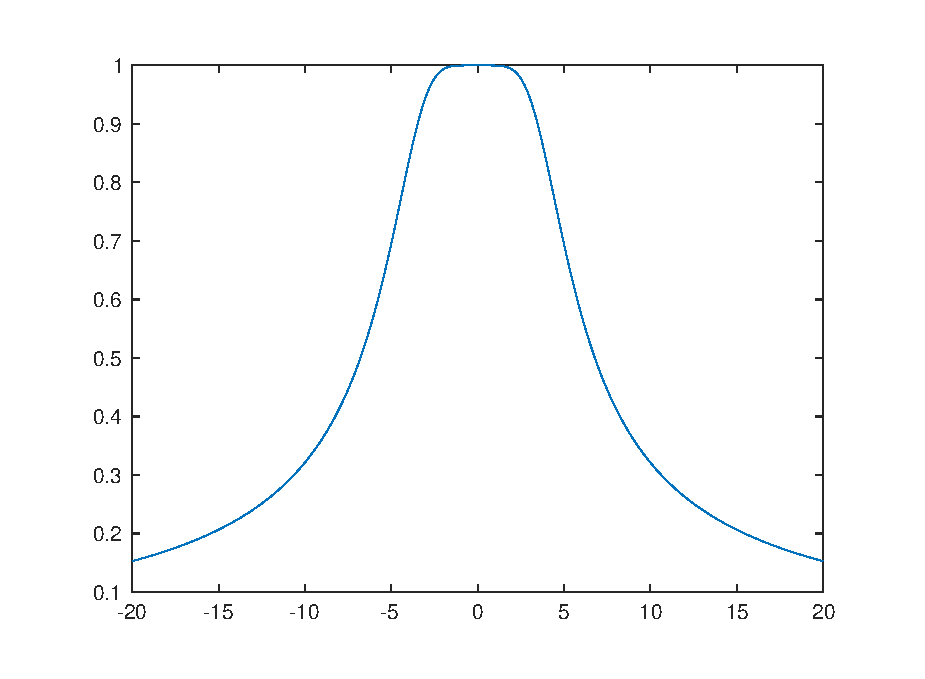
\includegraphics[width=0.3\textwidth]{figures/11-266.eps}
\end{figure}

注意到$R(z)$的极点约为$\lambda_1\approx 2.6811+3.0504\mathbf{i}$,$\lambda_2\approx 2.6811-3.0504\mathbf{i}$,$\lambda_3\approx 3.6378$,都具有正实部,因此根据定理11.256,该方法是A稳定的。再根据定理11.260,得该方法是L稳定的。

\section*{XXI. Exercise 11.278 (隐式中点法的Butcher表与B稳定性)}

\;\;\;\;\;\;设
\begin{equation*}
    U^{n+1}=U^n+ky_1
\end{equation*}

代入原始公式得到:
\begin{equation*}
    y_1=f\left(\frac{U^n+U^{n+1}}{2},t_n+\frac{k}{2}\right)=f\left(\frac{k}{2}y_1,t_n+\frac{k}{2}\right)
\end{equation*}

上述两式即构成隐式中点法的标准形式,其Butcher表为:
\begin{table}[H]
    \centering
    \begin{tabular}{l|l}
        $1/2$ & $1/2$\\ \hline
        & $1$
    \end{tabular}
\end{table}

注意到$\mathbf{e}^{n+1}=\mathbf{U}^{n+1}-\mathbf{V}^{n+1}=\mathbf{e}^n+k\mathbf{W}$,其中
\begin{equation*}
    \mathbf{W}= \mathbf{f}\left(\frac{\mathbf{U}^n+\mathbf{U}^{n+1}}{2},t_n+\frac{k}{2}\right)
    +\mathbf{f}\left(\frac{\mathbf{V}^n+\mathbf{V}^{n+1}}{2},t_n+\frac{k}{2}\right) .
\end{equation*}

从而
\begin{equation}
    ||\mathbf{e}^{n+1}||^2 = \left\langle \mathbf{e}^n+k\mathbf{W}, \mathbf{e}^{n+1} \right\rangle= \left\langle \mathbf{e}^n, \mathbf{e}^{n+1} \right\rangle + k \left\langle \mathbf{W}, \mathbf{e}^{n+1} \right\rangle
\end{equation}

注意到:
\begin{equation*}
    \mathbf{e^n}+\mathbf{e^{n+1}}=\frac{\mathbf{U}^n+\mathbf{U}^{n+1}}{2} - \frac{\mathbf{V}^n+\mathbf{V}^{n+1}}{2}.
\end{equation*}

因此,由吸引系统(contractive ODE system)的性质$\mu=0$,有
\begin{equation*}
    \left\langle \mathbf{e^n}+\mathbf{e^{n+1}},  \mathbf{f}\left(\frac{\mathbf{U}^n+\mathbf{U}^{n+1}}{2},t_n+\frac{k}{2}\right)
    +\mathbf{f}\left(\frac{\mathbf{V}^n+\mathbf{V}^{n+1}}{2},t_n+\frac{k}{2}\right) \right\rangle\leq \mu||\mathbf{e^n}+\mathbf{e^{n+1}}||^2=0
\end{equation*}

从而有:
\begin{equation*}
    \left\langle \mathbf{W},\mathbf{e}^{n+1} \right\rangle \leq - \left\langle \mathbf{W},\mathbf{e}^{n} \right\rangle
\end{equation*}

代入(1)式得:
\begin{align*}
    ||\mathbf{e}^{n+1}||^2&\leq \left\langle \mathbf{e}^n, \mathbf{e}^{n+1} \right\rangle - k \left\langle \mathbf{W}, \mathbf{e}^{n} \right\rangle\\
    &= \left\langle \mathbf{e}^n, \mathbf{e}^{n+1}-k\mathbf{W} \right\rangle = \left\langle \mathbf{e}^n, \mathbf{e}^{n} \right\rangle
\end{align*}

从而得到$||\mathbf{e}^{n+1}||\leq ||\mathbf{e}^n||$,即B稳定性。

\bibliographystyle{plain}
\bibliography{reference}

\end{document}

%%% Local Variables: 
%%% mode: latex
%%% TeX-master: t
%%% End: 
